\documentclass[Royal,times,sageh]{sagej}

\usepackage{moreverb,url,natbib, multirow, tabularx}
\usepackage[colorlinks,bookmarksopen,bookmarksnumbered,citecolor=red,urlcolor=red]{hyperref}



% tightlist command for lists without linebreak
\providecommand{\tightlist}{%
  \setlength{\itemsep}{0pt}\setlength{\parskip}{0pt}}



\usepackage{setspace}


\begin{document}


\setcitestyle{aysep={,}}

\title{Network Regression on Cosponsorship and Religion in United States
Congress}

\runninghead{Dionne \& Liftman.}

\author{Natalie Dionne\affilnum{1}, Naomi Liftman\affilnum{2}}

\affiliation{\affilnum{1}{Department of Government, Smith
College}\\\affilnum{2}{Department of Statistical and Data Science, Smith
College}}

\corrauth{Naomi Liftman}

\email{\href{mailto:nliftman@smith.edu}{\nolinkurl{nliftman@smith.edu}}}

\begin{abstract}
Given the recent surge in identity politics, we explore the effects
religion has on the legislative agenda. In mapping all 70,000 pieces of
legislation from the 112th (2011-2013) and the 117th (2021-2023)
Congress, we infer a series of political relationships among
legislators, which we then use to test; (1) If religion influences
cosponsorship in the congressional network? (2) If that influence has
changed in the last 10 years? We find evidence that in recent years,
religious identity affects legislature's cosponsorship behavior. This
analysis suggests a positive trend in religion-based polarization in the
United States Congress.
\end{abstract}

\keywords{Cosponsorship, Networks, Religion, Polarization}

\maketitle

\singlespacing

\citep{mitchell_faith_2021}

\hypertarget{introduction}{%
\section{Introduction}\label{introduction}}

\doublespacing

~~Extensive literature supports the importance of cosponsorship as the
core activity in building the legislative agenda. As Schiller (1995)
outlines, sponsorship is one of the few legislative activities which
legislators have almost total control. Legislatures can decide to
introduce and support legislation that appeases their constituents,
progresses their political career, and initiates institutional change on
a variety of policies. While legislators can be thought of as individual
sponsoring and cosponsoring bills, when combined the collaborative
process of agenda setting reflects shared interests and communal values.
The agenda setting stage is believed to be critical in the legislative
process due to its ability to control or manage what issues gain
government attention.

As cosponsorship is the most used tie in the legislative network, there
is a growing body of literature that explores a variety of identity
based characteristics on cosponsorship networks. This research has
focused primarily on political identities (i.e.~partisanship and
political ideology) {[}should i cite who?{]} and visible identity
characteristics (i.e.~age, race, gender, and ethnicity). Both have
provided extensive support of Huckfeldt's (1984) claim that one's
community and one's individual characteristics influence their political
actions.

However, existing scholarship falls short on researching the effects of
religious affiliation on the congressional cosponsorship network. Given
its intrinsic function as a core component of an individual's identity
and its known effect on political ideology (Mctague \& Pearson-Merowitz
2013), there is a theoretical framework that religion influences
legislators actions. This paper provides empirical evidence on how the
congressional cosponsorship network is affected by legislators'
religious identity.

In this paper, we examine the United States 112th Congress (2011-2013)
and the 117th Congress (2021-2023). Data on sponsorship and
cosponsorship (roughly 30,000 bills each session) is used in conjunction
with network analysis to model the influence of religion in each
respective session. We then cross compare the resulting networks to
understand how the effect of religious affiliation on congressional ties
has changed over the past ten years. With this, we also contribute to
the existing body of literature on recent trends in polarization,
specifically the growing political division created by religion.

\hypertarget{literature-review}{%
\section{Literature Review}\label{literature-review}}

\hypertarget{co-sponsorship-used-to-model-congressional-networks}{%
\subsection{Co-Sponsorship used to Model Congressional
Networks}\label{co-sponsorship-used-to-model-congressional-networks}}

~~Across disciplines, there is extensive literature supporting the
effects of social networks, characterized by friendship, support,
acquaintanceship, and communication on individual decisions. Rice (1927)
began the earliest attempts of modeling the social network of United
States Congressional Representatives by analyzing roll-call votes.
Roll-calls are simply the act of voting yes or no on a measure presented
before the Congress. Studies have found that this action is more
reflective of the individual's ideology or preference in the moment,
rather than having any significant pressure from a network (Fowler
2006). Scholarship since have used a variety of connectors to tie
legislatures; participant interviews, questionnaires, social media
interactions, campaign finance, presence at common events, and most
significantly to this study; cosponsorship.

Cosponsorship has become the most common strategy for indirectly
inferring legislators' relations and has been used to examine both state
and federal bodies throughout the world (Neal 2020). The bill
sponsorship system in the United States is designed with one ``primary
sponsor'' which is the legislator who introduces the bill. Despite the
fact that some bills are coauthored, there is only one formal primary
sponsor, the rest of the legislators who sign their support to the bill
are cosponsors. Schiller (1995) argues that bill sponsorship is one of
the few activities over which legislatures have almost total control.
This is the means by which legislators can introduce and support
legislation that appeases their constituents, progresses their political
career, and enact change on a variety of policies.

While ``legislators can be thought of as individually sponsoring and
cosponsoring measures, agenda setting as an institutional exercise is an
activity that reflects shared interests and certainly involves
interaction among legislators.'' Bratton \& Rouse (2011, pg424)
Literature further defends the idea that legislative power of
cosponsorship through its ability to set the agenda. Agenda setting is
the process by which policymakers effectively control or manage the
issues that receive political attention. While most bills do not pass
and less than 4\% receive cosponsors, the sponsorship process determines
what issues are on the table and therefore subject to institutional
change.

Using cosponsorship data as a tie to connect legislatures in the
Congressional network was largely pioneered by Fowler (2006) when he
discovered that analysis normally focuses on which bills legislatures
will support rather - than which legislatures will support which
legislatures. He then used social network analysis to examine
cosponsorship from 1973 to 2004 in the US Congress. Crafting a measure
of connectedness, he found that well-connected legislators are more
successful at passing amendments and gaining support in roll-call votes,
a frequent indicator of political influence. Gross (2007) uses a
multilevel approach to examine potential social factors on the varying
odds of cosponsorship between legislators in the network. He finds that
ideological similarity, being from the same state, and sharing committee
assignments increase the likelihood that a legislature will support a
colleague's bill (further supported by Zhang et al., 2008; Bernhard and
Sulkin, 2009; Cho and Fowler, 2010).

\hypertarget{co-sponsorship-used-to-model-congressional-networks-as-it-relates-to-identity}{%
\subsection{Co-Sponsorship used to Model Congressional Networks as it
Relates to
Identity}\label{co-sponsorship-used-to-model-congressional-networks-as-it-relates-to-identity}}

~~There is also a growing body of evidence that core characteristics of
a legislature's identity has an effect on the congressional network.
``This tendency, often described as ``birds of a feather flock
together,'' is prevalent across social networks in a variety of
contexts, from friendship groups to schools and businesses'', creating a
strong likelihood of its prevalence in congress (Craig et al 2016 pg 2).
This connection to the congressional network began with Huckfeldt
(1984), who originally theorized that one's community and individual
characteristics influence the way they interact in the political sphere.
This laid the foundation to an investigation into the effects of race,
gender, and ethnic identity on cosponsorship in the congressional
network.

The existing literature on the effects of homophily (similar
characteristics such as race, gender, and ethnicity) are somewhat split
by majority and minority status. Bratton \& Rouse (2011) examine
numerous social determinants within the cosponsorship network of state
legislatures. Their conclusions on the effects of gender and race on
legislators' general propensity to cosponsor varied by state. They found
strong correlations between homophily and cosponsorship in Texas and
California but moderate effects in the other states of interest.
However, when they factored minority status into the equation they found
a strong correlation in every state legislature. This means that women,
Latinos, and African-Americans were relatively more likely to endorse
the proposals of others who shared their respective minority status.
While they can only hypothesize, Bratton \& Rouse suggest that Social
Identity Theory explains these results.

Barnes (2016) examines the structure of the legislature to see if women
are excluded from the ``men's club''. In doing so, provides extensive
background on what encourages women to collaborate in the political
sphere. Her analysis concludes that women cosponsor more legislation
than men and a larger proportion of their sponsors are women. This
provides evidence that women are relatively more likely to cosponsor
measures introduced by other women. Wojcik \& Mullenax (2017), using
survey based evidence from Brazil's Chamber of Deputies, argue that
female representatives engage in higher rates of intragender networking.
This means that women have more profuse and diverse legislative networks
than male representatives. Combined these findings support the idea that
networks are affected by gender identity.

Rocca \& Sanchez (2008) challenge those conclusions with regards to race
and ethnicity. They find that on average Black and Latino legislators
sponsor and cosponsor significantly fewer bills in Congress than do
Whites and non-Latinos, respectively. They attribute this conclusion to
the systematic disadvantages in resources and the resulting desire to
support one's own group. Craig et al (2016) study the U.S. House
cosponsorship network from 1981 through 2004, to highlight the reality
faced by minority groups. They find that Black and Latino members of
congress are at a comparative disadvantage of race-based assortative
mixing in the cosponsorship process. This literature supports the idea
that race and ethnic identity affect the congressional cosponsorship
network.

The findings for cosponsorship based on homophily are further explained
through the psychological principles of the Social Identity Theory.
Tajfel (1979) concluded that the process of categorizing oneself as a
group member creates a positively valued social identity. Once
allegiances have been set, individuals will allocate more resources to
the in-group to maximize the benefits they have over the out-group.
Psychologists in the years since have discovered this to be especially
true as it relates to minority groups - women, Latino, and
African-American legislators. Due to the systematic disadvantages the
individuals in these groups face they are more likely to support those
within their respective social group.

\hypertarget{existing-literature-on-religion-but-not-cosponsorship-religion-networks}{%
\subsection{\texorpdfstring{Existing Literature on Religion but
\emph{NOT} CoSponsorship / Religion
Networks}{Existing Literature on Religion but NOT CoSponsorship / Religion Networks}}\label{existing-literature-on-religion-but-not-cosponsorship-religion-networks}}

~~The literature on congressional cosponsorship networks is vast and
studies regarding the effects of gender, race, and ethnicity are
becoming increasingly more abundant. However, there is very little (if
not any) research on the ways in which religion influences the
congressional cosponsorship network. This is quite surprising.

Religion is a core component of a legislature's identity, for some as
intrinsic as their sex or race, and for others entirely intertwined with
their ideology. Given this nature, we should expect a legislator's
religious affiliation to have a significant effect on their political
decision. Research has shown it does. Mctague \& Pearson-Merowitz (2013)
highlight the ways in which religion affiliation can predict party
affiliation (with Jews representing the most liberal, Catholic and
Protestants representing the moderate, and evangelical Christians
representing the furthest right). They also explain that the recent
growth in partisan polarization over cultural and ideological issues
only increases the tendency to follow one's religion to a political
party. Religion is therefore an intrinsic identity that divides
individuals into an in-group and an out-group. This provides evidence
that religion has the potential to function exactly like sex, race, and
ethnicity.\\
With that we have created three hypotheses to fill the gap in literature
on religion within the congressional cosponsorship network.

\emph{H1: (general) Legislators will be more likely to cosponsor
measures sponsored by colleagues with the same religious affiliation.}

\emph{H2: (minority group) Those belonging to religious minority groups
will be relatively more likely to cosponsor measures introduced by
another members of the same religious minority (ie Jewish legislators
will be more likely to cosponsor bills introduced by other Jewish
legislators)}

\emph{H3 (increased polarization) There will be a stronger effect of
religion (measured by legislators being more likely to cosponsor
measures sponsored by colleagues with the same religious affiliations)
in the 117th Congress compared to the 112th Congress. }

\hypertarget{research-design}{%
\section{Research Design}\label{research-design}}

\doublespacing

~~There is a lack of research on how religion affects the relationships
between legislators, as discussed above, and this paper looks to address
this gap. To understand the relationships between members of congress we
use cosponsorship as a measure of positive relationships. Cosponsoring
another member's bill is a sign of shared morals, values, and opinions
in a directional manner as cosponsoring a person's bill is a sign of
support, which does not inherently mean that bills writer supports the
cosponsor. So our paper is using cosponsorship as a measure of
similarity and positive relationships between members of Congress.

Recently there has been evidence that polarization has increased as
culture wars and identity politics become more prevalent; however, very
few of these papers look at religion. So to understand how religion has
changed over time we are looking at the 112th and 117th congress'. These
congresses were chosen because the 112th ran from January 3, 2011 to
January 3, 2013, which was after the financial crisis but before the
election of Donald Trump. Thus it seemed to be a suitable `control' case
for how religion affects cosponsorship. Then the 117th congress was
chosen as it is the most recent congress to finish a full session
running from January 3, 2021 to January 3, 2023. So at the time of this
writing it is the most recent complete congress we can access
cosponsorship data on. These sessions are also direct mirrors of each
other with the 112th having a Democratic President and Senate with a
Republican House and the 117th having a Republican President and Senate
and a Democratic House. So both of these congresses have similar groups
of control in the separate branches.

We are using two sets of models to assess the effect of religion. The
first set of models is to assess (x) hypothesis. This model is a network
regression model as such: \[
consponsorship = B_1(relgion) + B_2(party) + B_3(ideology)
\]

and we expect religion to be statistically significant for the 117th
congress but not the 112th congress. We do not expect party or ideology
to be statistically significant, as they are simply controlling for
other factors that may affect cosponsorship.

The second set of models is to assess (x) hypothesis. For this we are
again running a network regression model, but this time with
similarities in religion being variables separate from the whole
religion variable: \[
cosponsorship = B_1(catholic) + B_2(jewish) + B_3(other) 
\]

\[
+ B_4(protestant )+ B_5(unknown)
\] and we expect Jewish and Other to be statistically significant as
these are the minority groups in congress. But we do expect both of
these categories to be statistically significant in both the 112th and
117th congress. We will also run this model with the controls of party
and ideology to see if they change the results: \[
cosponsorship = B_1(catholic) + B_2(jewish) + B_3(other) + B_4(protestant )
\] \[
+ B_5(unknown) + B_6(party) + B_7(ideology)
\]

\hypertarget{data-and-networks}{%
\subsection{Data and Networks}\label{data-and-networks}}

\doublespacing

~~We pulled data from three main sources to build two networks with
different edge level covariables of congresspeople: the Pew Research
Center, Congressional Website on Cosponsorship, and Voteview (which are
discussed in depth in the data collection section). The first network is
of the 112th Congress with every congressional member in that session
being a node. The second network is the exact same setup except with the
117th Congress. In both of these networks the ties are of cosponsorship
with a tie being a member cosponsoring another members legislation and
these ties are binary, directed, and exclude self-ties.

Within each of these two networks there are three edge level
covariables: religion, ideology, and party. Religion and party are both
binary undirected ties that exclude self-ties with ideology being the
same except being a weighted tie.

\hypertarget{dependent-variable}{%
\subsection{Dependent Variable}\label{dependent-variable}}

\doublespacing

~~The dependent variable in our model is \texttt{cosponsorship}, which
is measured as a binary and directed tie between two congresspeople.
Ties are binary with any example of cosponsorship between two members
given a 1 and the lack of the behavior given a 0. This paper considers
legislation to be any of the following proposals in both the House and
the Senate: Bill, Joint Resolution, Concurrent Resolution, and a Simple
Resolution. There is precedent for using all four of these types of
proposals as legislation(citation); however, we also use all of them as
this gives us the largest and most expansive amount of data to work
with.

In the 112th congress there are 531 members with a total of 31706 total
cosponsorship ties between members, with most members cosponsoring
multiple pieces of legislation (93.4 percent). There are only three
members cosponsoring no legislation. The member who cosponsored the most
legislation in the 112th was Stephen Fincher who cosponsored 200 bills.

In the 117th congress there are 535 members with a total of 35826 total
cosponsorship ties between members, with a slightly higher majority of
members cosponsoring multiple pieces of legislation than in the 112th
(96.6 percent). There are still two members who do not cosponsor any
legislation. In the 117th the member who cosponsored the most
legislation was Jennifer Wexton with 215 bills. Together across these
two congresses there is a large swath of legislation allowing us to get
a full picture of cosponsorship in these two sessions.

\hypertarget{independent-variables}{%
\subsection{Independent Variables}\label{independent-variables}}

\doublespacing

~~There are three independent variables used in our model:
\texttt{religion}, \texttt{ideology}, and \texttt{party}. While
\texttt{religion} is the one we are focusing our attention on, as there
is a large gap in the literature surrounding it, we decided to include
\texttt{ideology} and \texttt{party} as other independent variables as
we believe that religion, ideology, and party of members are intertwined
in the relationships that are formed.

\hypertarget{religion}{%
\subsection{Religion}\label{religion}}

\doublespacing

~~The first, and most important of our Independent Variables is
\texttt{religion}, which is measured using CQ Roll Call questionnaire
which asks members of the House and Senate identity based questions such
as their religion. With this, each member reported their religious
affiliation; however, there are a wide range of different religions
across Congress so we reduced these categories into smaller ones in
order to better analyze the effects.

In the 112th congress members reported 38 different religious
affiliations amongst them with only a slight decrease to 24 in the
117th. But many of these categories of religion either only include a
handful (or oftentimes only 1) of members or fall under broader
religious categories. To deal with this we used the
\href{https://www.pewresearch.org/religion/2021/01/04/faith-on-the-hill-2021/}{Pew
Research Centers} methodology to determine what religions could be
categorized under larger ones, and ended with five main religious
groups: Catholic, Protestant, Jewish, Other, and Unknown.

For the 112th congress we reduced 4 of the original religions categories
reported to Catholic: Anglican, Anglican Catholic, Roman Catholic, and
Unitarian. All four of these religions are either Catholic in and of
themselves, follow the same beliefs as Catholicism, or are an offshoot
of Catholicism. We then continued this process for the other four
categories. We reduced 25 religious categories to Protestant, 1
religious category to Jewish, 6 religious categories to Other, and 2
categories to Unknown. The most interesting category is Other with there
being Quakers, Nazarenes, Greek Orthodox, Mormon, Buddhist, and Muslim.

For the 117th congress there were 24 broad religious affiliations with 2
groups categorized as Catholic, 13 religious categories reduced to
Protestant, 1 to Jewish, six to Other and 2 to Unknown. The Other
category is made up of Unaffiliated, Buddhist, Hindu, Mormon, Muslim,
and Nondenominational. Across both sessions of congress when two members
belong to the same of these five groups they are given a 1 and they are
given a 0 if they belong to different groups. For breakdowns of members
into religious groups see Figure \ref{fig:plot}.

\hypertarget{ideology}{%
\subsection{Ideology}\label{ideology}}

\doublespacing

~~The second independent variable in our model is \texttt{ideology}, and
to measure ideological similarities between members we used DW-NOMINATE
scores. NOMINATE is an acronym for Nominal Three-Step Estimation and is
often used to quantify political ideologies of people, parties, and
political institutions. We will be using the first dimension, which is
measured on a scale from -1 to 1 on a liberal-conservative scale, as
this dimension quantifies a general political leaning without looking
too intricately at specific policies. On this scale a -1 describes an
extreme liberal and a 1 describes an extreme conservative.

In our model we calculated the absolute value of the difference between
DW-NOMINATE scores between members with members who were very similar in
ideology would have a close to zero score and members with extreme
ideological differences would be close to 2. For the 112th congress the
most liberal member was Barbara Lee with a score of -0.679 and the most
conservative member was Paul Broun with a score of 0.913. This is a
smaller range than the 117th congress, with an average score of 0.078,
which shows a conservative lean. The average difference between members
was 0.496.

For the 117th congress the members ranged in score from -0.811 on the
liberal end with Sylvia R. Garcia to 0.936 on the conservative end Tommy
Tuberville. The average of scores in the 117th congress is 0.061, which
shows a slight conservative lean in this session. The average difference
between members was 0.519, which is relatively large and an increase
from the 112th congress. This may point towards an increase in
polarization discussed in other papers.

\hypertarget{party}{%
\subsection{Party}\label{party}}

\doublespacing

~~The final independent variable in our model is \texttt{party} which
refers to the political party of the members. This is measured as either
Republican, Democrat, or Independent; however there were only two
independents for both sessions respectively so we recategorized each of
them according to what their beliefs most closely aligned with.

In the 112th congress there were two members who identified themselves
as Independents which were Joseph I. Lieberman and Bernard Sanders. Both
of these members have sincere left leanings, as confirmed by their
DW-NOMINATE scores of -0.205 and -0.538 respectively. Because of these
leftist inclinations we recategorized both of them as Democrats to allow
for a more complete analysis.

In the 117th congress there were again two people who identified
themselves as Independents: Angus King and Bernard Sanders. As we have
already discussed Sanders was recategorized as a Democrat in the 112th
congress and the same process was conducted to recategorize him as a
Democrat again. We did the same process with Angus King, and after
confirming his DW-NOMINATE score of -0.161 we recategorized him as a
Democrat.

If two members are a part of the same party they receive a 1 and if they
are not they receive a 0. So if both members are Democrats then they
will receive a 1 and if both members are Republicans they will also
receive a 1; however if there is any difference such as one Republican
and one Democrat then they will receive a 0.

\hypertarget{data-collection}{%
\subsection{Data Collection}\label{data-collection}}

\doublespacing

~~To aggregate data on cosponsorship we used the \texttt{incidentally}
package which automatically goes through congress's
\href{https://www.congress.gov/}{website} to get data on legislators'
bill sponsorship and cosponsorship activities. To aggregate data on the
religion of members we used two documents collected by the Pew Research
Center for both the
\href{https://www.pewresearch.org/religion/2021/01/04/faith-on-the-hill-2021/}{117th}
and the
\href{https://www.pewresearch.org/religion/2011/01/05/faith-on-the-hill-the-religious-composition-of-the-112th-congress/\#a-look-back}{112th}
congress. These documents from the Pew Research Center also had
information on the party affiliation of members, which allowed us to
aggregate the data easier. Then for the other independent variable of
DW-NOMINATE we used the website
\href{https://voteview.com/data}{voteview} to collect each member's
scores.

The only issues with our data collection were that there were a few
members of congress who were present in other datasets but not in the
initial pull of religions. Since we based our network off of the
religion datasets, we were required to remove around 3-5 senators from
the cosponsorship and DW-NOMINATE datasets.

\hypertarget{methods}{%
\section{Methods}\label{methods}}

\doublespacing

~~After running our two sets of models we were pleased with many of the
results. For the first set of models, which looked to predict if
religion affected cosponsorship in members of Congress we found that it
did affect them during the 117th session but not for the 112th. Table
\ref{table1} shows our findings for the 117th, which are that we have
statistically significant evidence (alpha = .05, p-value = 0) that
religion is affecting cosponsorship of the 117th congress after
accounting for party and ideology. However, we do not find the same
evidence that there is an effect of religion and cosponsorship in the
112th congress. See table \ref{table2} and \ref{table1} for results of
the 112th and 117th congress respectively.

For the second set of models, which looked to assess specific religions
to see if they affected cosponsorship, we found that for the 112th
congress none of the religious groups were statistically significant
(see table \ref{table3}). This means that in the 112th congress we do
not have evidence that minority religious groups in congress were more
likely to cosponsor legislation with other legislators in their same
group. We also did not find evidence that non-minority religions,
Catholic and Protestant, were more likely to cosponsor legislation with
fellow Catholic or Protestant members. We also ran this model with the
inclusion of the control variables of party and ideology, but the
results did not change, and thus are only including the model without
them to lower our R-squared.

However, when we moved to the 117th congress we found that all of the
religious groups were statistically significant (see table
\ref{table4}). This means that for this congress we have evidence at the
.05 alpha level that people are more likely to cosponsor legislation
with other members within their religious group, no matter if they are a
minority or majority religion. We again also ran this model with the
inclusion of the control variables of party and ideology, but the
results did not change.

\hypertarget{conclusion}{%
\section{Conclusion}\label{conclusion}}

~~As individual identity is becoming increasingly more politicized and
therefore polarized, it is important to understand its effects on the
legislative agenda. In this paper, we have focused on the United States
112th Congress (2011-2013) and the 117th Congress (2021-2023) to
understand how the effect of religious affiliation on congressional ties
has changed over the past ten years. This analysis provides empirical
evidence on how the congressional cosponsorship network is affected by
legislators' religious identity.

Given the split result by congressional terms, two major conclusions can
be drawn from this research. First, the network analysis of the 117th
Congress provides evidence that religious affiliation has an effect on
the cosponsorship network. This effect is notably significant regardless
of minority and majority status. Practically, this means legislators
will be more likely to cosponsor measures sponsored by colleagues with
the same religious affiliation. These findings imply the effects of
religion are comparable to other key identity characteristics as
discovered in existing reports {[}site most relevant sources{]}.

Secondly, the inconclusive results for the 112th Congress provide
evidence that religion did not have a statistically significant effect
on the cosponsorship network in 2011 to 2013. While this challenges the
general hypothesis that religion would impact the ways in which
legislatures collaborate, it does mean religion's effect on the
congressional network is a relatively new phenomenon. This, in turn,
provides evidence for increased political polarization based on
religion.

While this study is not the first to limit the scope of congressional
terms {[}see Bratton \& Rouse and others{]}, it is important to note
when establishing trends. Future research should focus on the 10 years
between our findings to find the exact shift of religion's influence on
congressional cosponsorship.

Even despite this limitation, there are substantial practical
implications for this paper. Firstly, it bridges the gap between
existing literature on general cosponsorship and the effects of identity
on congressional behavior. Our paper builds on both to say that religion
influences the ways in which legislatures collaborate and therefore
collectively build the legislative agenda. This provides a new avenue of
research for future scholars. More notably, this paper points to the
future of Congressional politics, eliciting more questions about the
mechanisms that lead to polarization. How is the greater public impacted
when legislatures are influenced by religion when deciding what issues
receive government attention?

\hypertarget{bibliography}{%
\section{Bibliography}\label{bibliography}}

\hypertarget{tables-figures}{%
\section{Tables, Figures}\label{tables-figures}}

\begin{figure}

{\centering 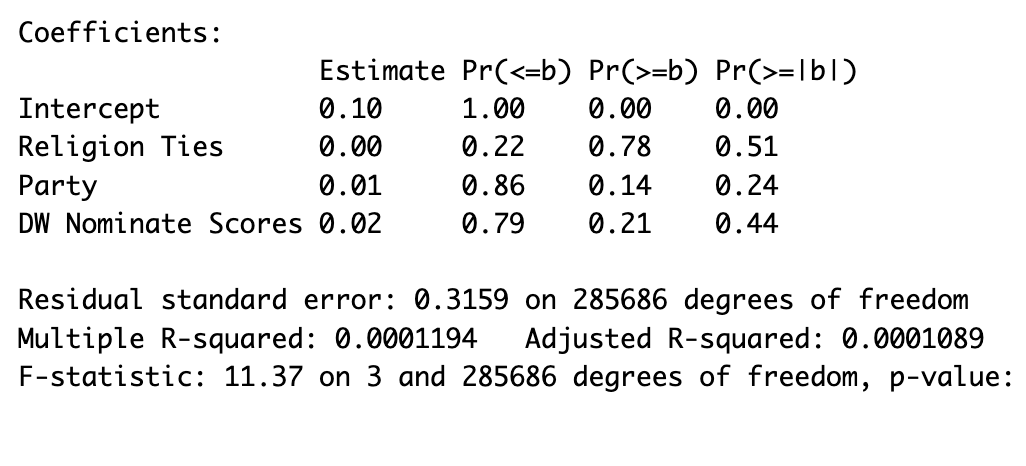
\includegraphics[width=0.7\linewidth]{images/112th_religion_firstmodel} 

}

\caption{Model for measuring religious effects of cosponsorship in the 112th session.\label{table1}}\label{fig:table1}
\end{figure}

\begin{figure}

{\centering 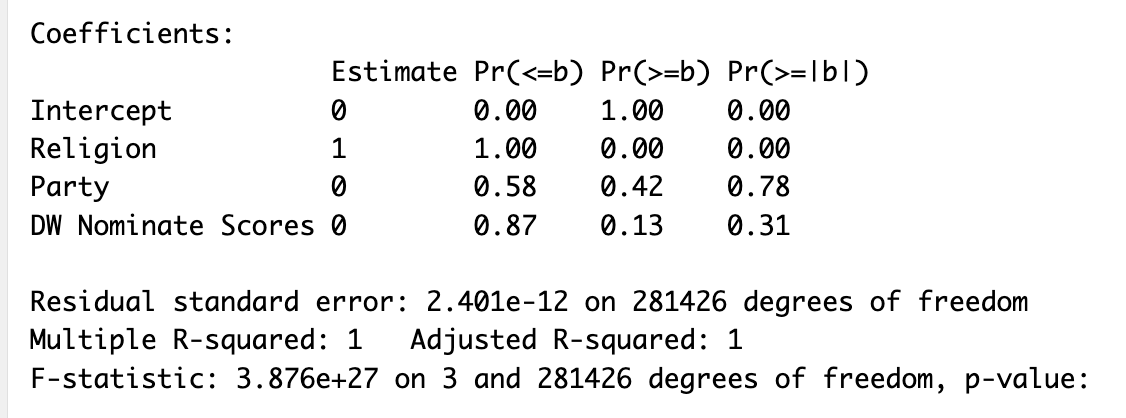
\includegraphics[width=0.7\linewidth]{images/117th_religion_firstmodel} 

}

\caption{Model for measuring religious effects of cosponsorship in the 113th session. \label{table2}}\label{fig:table2}
\end{figure}

\begin{figure}

{\centering 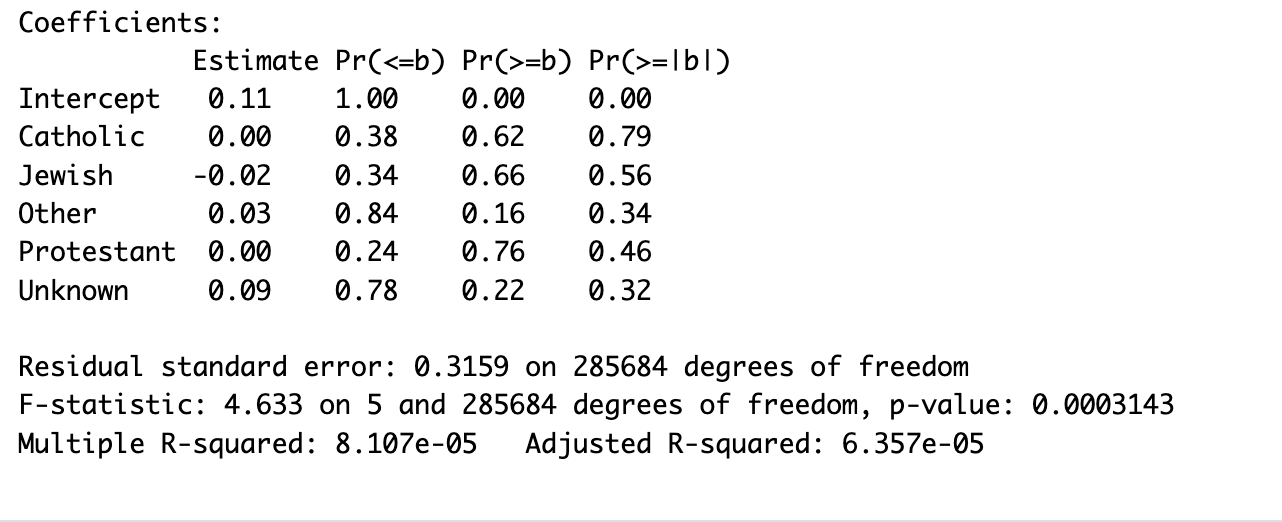
\includegraphics[width=0.7\linewidth]{images/112th_religion} 

}

\caption{Model for measuring effects of specific ingroup behaviors of 112th session. \label{table3}}\label{fig:table3}
\end{figure}

\begin{figure}

{\centering 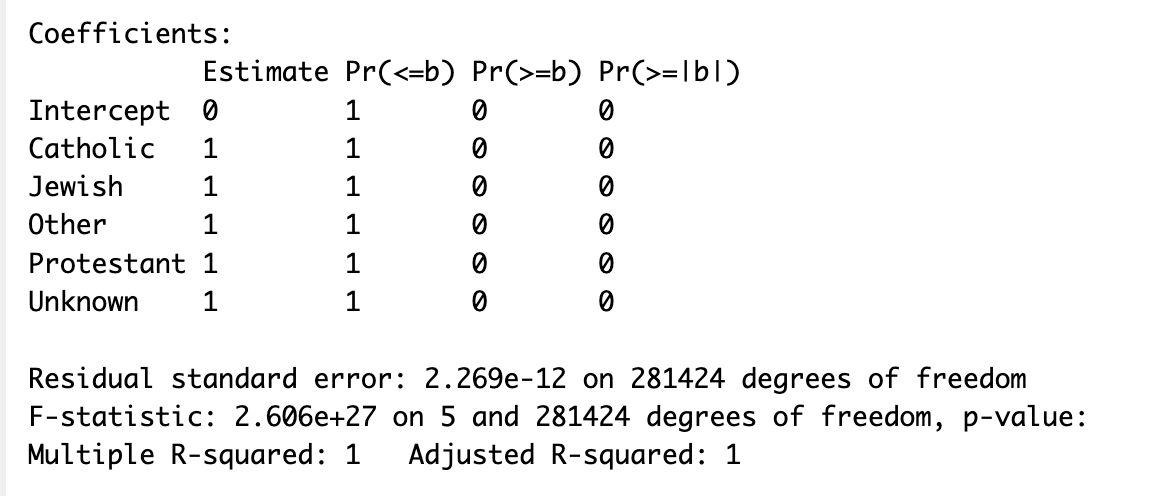
\includegraphics[width=0.7\linewidth]{images/117th_religion} 

}

\caption{Model for measuring effects of specific ingroup behaviors of 117th session.\label{table4}}\label{fig:table4}
\end{figure}

\begin{figure}
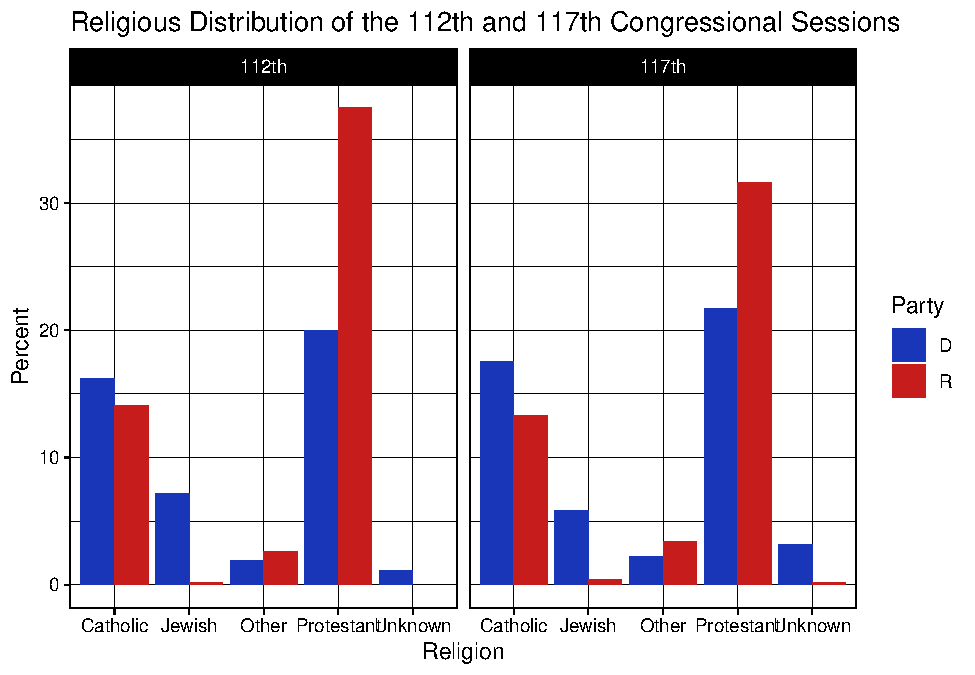
\includegraphics[width=1\linewidth]{final_reprorrt_files/figure-latex/plot-ref-1} \caption{\label{fig:plot}}\label{fig:plot-ref}
\end{figure}

\bibliographystyle{sageh}
\bibliography{citations}


\end{document}
